\newpage
\chapter{Artificial Neural Networks}

Artificial neural network models take their inspiration from the brain.

The brain is an information processing device (very different from a computer) that surpasses current engineering products in many domains (e.g., vision, speech recognition, learning and many others).

It is composed of a very large number of processing units, the neurons, ($10^{11}$) operating in parallel and largely connected. Neuron connections are called synapses, and each neuron connects to around $10^4$ other neurons, all operating in parallel.

In a computer, the processor is the active component while the memory is mainly separate and passive, but it is believed that in the brain, both the processing and memory are distributed together over a network.

The structure of the brain gave inspiration to a theoretical approximation \cite{ml}, where a collection of processors with a small amount of local memory implements a fixed function and executes the same instructions but each processor load different values so that they can do ``different things'' (e.g. attributing more importance to certain patterns of data). In this way, the main operation - whatever it is - can be distributed over such processors.

This theoretical approximation is called \textbf{Neural Instruction Multiple Data} (NIMD) machine, where each processor corresponds to a neuron, local parameters correspond to its synaptic weights, and the whole structure is a \textbf{neural network}.

The process through which local parameters are updated in order to achieve the task is called \textbf{learning}.

There are two types of learning: supervised and unsupervised. Both in supervised and unsupervised approach, learning is guided by samples of data.

In \textbf{supervised learning}, samples are associated to some labels that determine their class/score/desired feature; the networks should learn a mapping between them and reflects it on unknown data.

Regression and classification are two types of problems of supervised learning.

In classification problems, the aim is to find a mapping from the input to a discrete or categorical output, while in regression problems, the input has to be mapped toward a numerical/continuous output.

In \textbf{unsupervised learning}, labels are not provided and the network should discover the patterns and regularities within the samples to learn.

\section{Feed Forward Neural Networks}

There are many types of neural networks, but in this thesis I will cover in detail just feed forward neural networks due to the fact that they are used in DRMM \cite{drmm} and, in the context of that experiment (a task of ad hoc retrieval with a small data collection) have been proved to be effective compared to other approaches (e.g. convolutional in \cite{cdssm}).

\subsection{The perceptron}

The perceptron is the basic processing element of an artificial neural network. It takes as input a vector $\vec{x} \in \mathbb{R}^d$ from $\mathcal{X}$ and another vector of \textit{connection weights} $\vec{w} \in \mathbb{R}^d$.

Suppose that there is a dataset that contains some data samples $\mathcal{X}$ and their labels $\mathcal{Y}$.

The output $y$, in the simplest case, is a linear combination of the two:

\begin{equation}
\label{eq:lin}
\tag{linear combiner}
y = \sum_{j = 1}^d (w_j \cdot x_j) + w_0
\end{equation}

where $w_0$ is the \textit{intercept value}, independent from data and it's useful to give preference to a
class over another (e. g., in case of unbalanced datasets).

The perceptron (in equation \ref{eq:lin}) defines a hyperplane (a generalization of the two-dimensional plane in a space with $n$ dimensions) that in a binary classification problem can split the input space into two parts: the half-space with positive samples and the half-space with negative samples.

So, the perceptron can separate two classes by checking the sign of the output (defined as \textit{threshold function}).

Under supervised learning, it is necessary to compare the prediction $y$ to the label (desired output) $y' \in \mathcal{Y}$ associated to $x$ in the dataset and define a cost function (loss) $\mathcal{L}$ that indicates how well the perceptron performed.

Such loss function is used to define the total error, given by computing the loss function over all instances in $\mathcal{X}$ received by the perceptron:

\begin{equation}
E(\mathcal{W}| \mathcal{X}) = \sum_{i = 1}^{|\mathcal{X}|} \mathcal{L}(y_i', y_i)
\end{equation}

where $\mathcal{W}$ are the connection weights.

For instance, one pretty common loss function is the \textbf{mean squared error} function:

\begin{equation}
    \mathcal{L}(y, y') = (y - y')^2
\end{equation}

If the error function is differentiable, a technique generally used to minimize it is \textbf{gradient descent}. The aim is to find $\mathcal{W}^*$ such that $\mathcal{W}^* = \arg \min_{\mathcal{W}} E(\mathcal{W}| \mathcal{X})$.

The gradient descent algorithm iteratively (over a fixed number of \textit{training epochs}) updates weights using the following update equation:

\begin{equation}
\tag{gradient descent}
w_{j, t+1} = w_{j,t} - \eta_t \cdot \frac{ \partial \mathcal{L}}{\partial w_j} \qquad \forall j=0 \dots d
\end{equation}

where $t$ is the epoch number and $\eta_t$ is a learning rate that typically declines with t.

In order to evaluate a neural network performance, the dataset available is usually split into two parts: training and testing (e.g. 50-50\%). A fraction of the training part is then used as validation set to evaluate the network without updating its parameters. This is useful in order to avoid overfitting (described in the following).

When samples from the training set are selected randomly, a variant of gradient descent is used, called \textit{stochastic} (or ``on-line'') gradient descent.

In case of large dataset, the estimation of the true gradient at each sample would be too expensive to compute. A common solution consists in the use of \textbf{mini batches} of data: the gradient is computed over small random batches of data samples.

\subsection{Multi Layer Perceptron (MLP)}

A perceptron with a single layer of weights, as described in the previous section, can only approximate linear functions; however this limitation does not apply to networks with intermediate or hidden layers between the input or output.
 
Such multilayer perceptrons (MLP) can approximate nonlinear functions of the input.

Input $x$ is fed to the input layer, then the ``activation'' propagates in the forward direction, and the outputs $z_h$ of the hidden units are computed. This type of networks are called ``feed forward'' neural networks.

For instance, the feed forward network represented in figure \ref{fig:ffnn} uses the \textit{sigmoid} as non linear activation function in each hidden unit:

\begin{equation}
    \tag{Sigmoid function}
    z_h = \frac{1}{1 + exp(- \sum_{j=1}^d w_{hj} x_j + w_{h0})} \quad h = 1, \dots, H
\end{equation}

The hidden units make a nonlinear transformation from the $m$-dimensional input space to the $H$-dimensional space spanned by the hidden units, and then, in this space, the third (and final) output layer implements a linear function:

\begin{equation}
    y_i = v_i^T \cdot z = \sum_{h = 1}^H v_{ih} \cdot z_h + v_{i0}
\end{equation}

\begin{figure}[H]
  \centering
  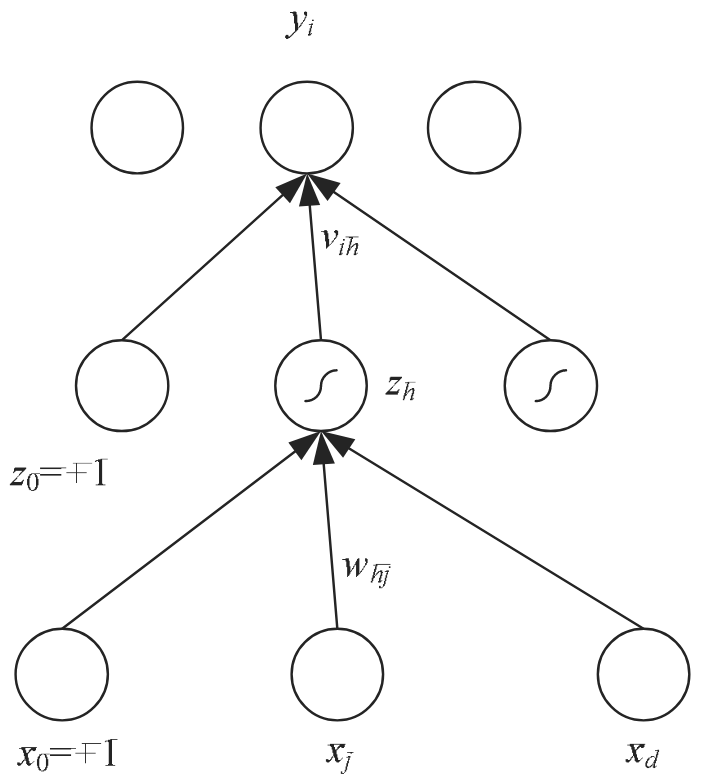
\includegraphics[width=0.5\textwidth]{MLP.png}
  \caption{The structure of a MLP with $d$ input units ($x_0, \dots, x_d$) and $H$ hidden units ($z_0, \dots, z_H$) where $x_0$ and $z_0$ are the bias units. $w$ and $v$ are the weights for the first and the second layer respectively (image source: \cite{ml}).}
  \label{fig:ffnn}
\end{figure}

Sigmoid is the continuous, differentiable version of thresholding and thus, gradient descent is suitable for learning process in MLP.

Another nonlinear function that can be used is the hyperbolic tangent function, \textit{tanh}, which ranges from $-1$ to $+1$, instead of $0$ to $+1$ (used in \ref{chap:drmm}).

Because of the nonlinearity, such error function has many minima and gradient descent converges to the nearest minimum. To be able to assess expected  error,  the  same  network  is  trained  a  number  of  times  starting from different initial weight values, and the average of the validation error is computed.

\subsection{Complexity}

A MLP with $d$ input units, $H$ hidden units, and $K$ outputs has $H \cdot (d+1)$ weights in the first layer and $K \cdot (H+1)$ weights in the last layer (including the bias term).

Let $e$ be the number of training epochs for the MLP. Then, $H$ and $e$ are two free parameters (in this simplified setting) - also known as hyper parameters (but there can be others, e.g. mini batches size).

The tuning of these parameters aim to minimize the generalization error (i.e. the error on the test set).
A simple model with abundant data can generalize well, while a complex model with fewer examples typically cannot, as it tend to overfit.

A similar behavior occurs when training is continued  too long: the training error decreases, but the generalization error starts to increase beyond a certain point. This problem can be alleviated by \textit{stopping early} the learning process.
\todo{riportare figura?}
There are many factors that influence whether a model will generalize well and some of them are: the number of tunable parameter; the values taken by the parameters and the number of training examples.

\subsection{Overfitting / Underfitting problem and regularization}

\textbf{Underfitting} happens when a model does not have the capacity to fully learn the data while \textbf{overfitting} occurs when a model is too complex and does not generalize well (or even just memorize the training data).

The ideal fit should be the purpose of a neural network, so that it does not underfit neither overfit (see figure \ref{fig:overfitting}).

\begin{figure}
  \centering
  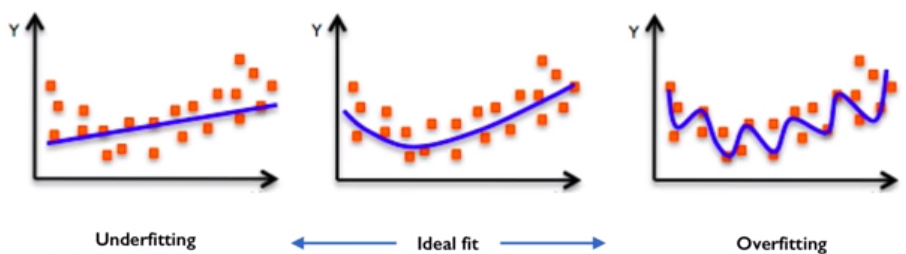
\includegraphics[width=0.9\textwidth]{overfitting.png}
  \caption{Underfitting, ideal fit and overfitting, source \url{pingax.com/wp-content/uploads/2014/05/underfitting-overfitting.png}}
  \label{fig:overfitting}
\end{figure}

In order to achieve this result, \textit{regularization} is often used. It is a set of techniques that constraint the optimization problem to discourage complex models. Some examples:

\begin{itemize}
 \item \textbf{Dropout}: randomly set some activation to zero. This forces the network to not rely on any particular node, and encourages it to explore different patterns on input data.
 \item \textbf{Early stopping}: stops the training before it overfits the data by monitoring a given metric (e.g. validation loss).
\end{itemize}

When the dataset available is too small, it can be exploited through k-fold cross validation so that each example in it is used both for training and (exactly once) for validation.

With K-fold cross-validation, the dataset is partitioned into k parts. Then, k-1 parts are used as training set and the remaining part is used as validation set. This process is repeated k times so that each part is used exactly once as validation set.
The k results can then be averaged to produce a single estimation.

It is often used for parameters tuning: k-fold cross validation is typically performed several times for different set of values associated to the parameter(s) to estimate.

\subsection{Universal approximation theorem}

In 1989 Hornik, Stinchcombe and White proved an important result: a MLP with one hidden layer can learn any nonlinear function of the input.

There are some caveats in this statement to consider: the number of hidden units may be infeasibly large; the resulting model may not generalize and there are no instructions on how to build/recognize such network.

\begin{figure}[H]
  \centering
  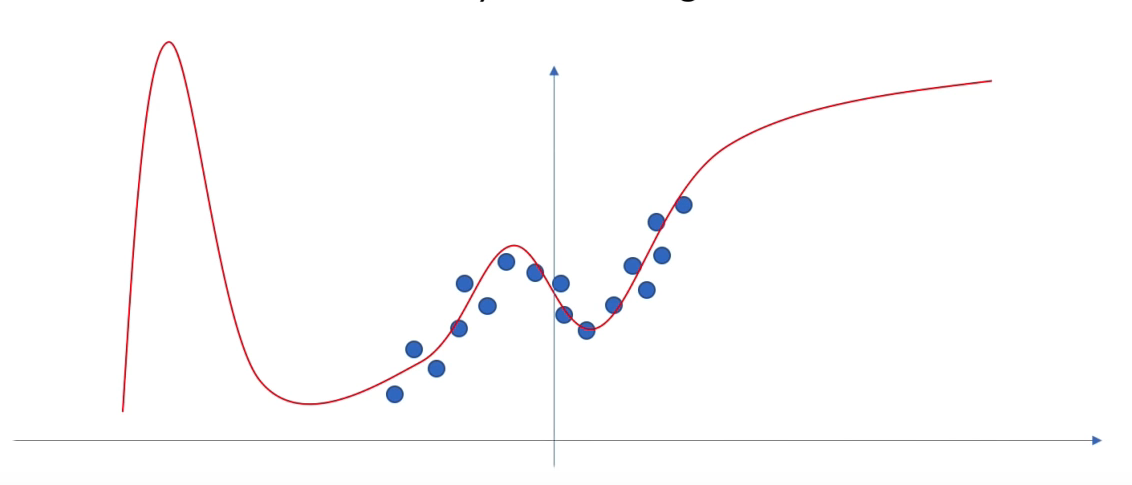
\includegraphics[width=0.9\textwidth]{func_approx.png}
  \caption{Training and test data problem}
  \label{fig:hist_ex}
\end{figure}

Neural networks are excellent function approximations, but there is a huge
problem: as long as they have training data, they may be perform well, but
there is no guarantee on their performance outside that data.

\section{Neural networks limitation}

The main advantage of neural network lies in their ability to outperform nearly every other machine learning algorithm, but this goes along with some disadvantages. They are:

\begin{itemize}
 \item very data hungry;
 \item computationally intensive;
 \item easily fooled by adversarial examples;
 \item poor at representing uncertainty;
 \item (sometimes) uninterpretable black boxes;
 \item difficult to optimize: there could be many factors to consider, depending on the task;
 \item difficult to model: often they requires expert knowledge to design, fine tune architectures.
\end{itemize}
